\chapter{Repaso acumulativo, simulacros y reto final}

\begin{theorybox}{Funcion de este bloque}
Este capitulo no nace de una fila concreta de la matriz de cobertura, sino como cierre original
del libro para recombinar tecnicas de \texttt{C01-C09}. Su objetivo es entrenar diagnostico,
eleccion de metodo, control de errores y trabajo con tiempo limitado.
\end{theorybox}

\begin{methodbox}{Ruta recomendada}
\begin{enumerate}
  \item Haz primero el diagnostico sin mirar apuntes.
  \item Vuelve al capitulo origen cuando detectes un fallo de base.
  \item Usa la hoja mixta para practicar cambios de tecnica.
  \item Reserva los simulacros para una sesion cerrada con tiempo real.
  \item Cierra con el reto final y anota en la tabla de seguimiento que bloque necesita mas
  consolidacion.
\end{enumerate}
\end{methodbox}

\section{[R10.S01] Diagnostico inicial}

\subsection*{Objetivo}
Comprobar en poco tiempo si siguen activos los automatismos basicos de dominio, ecuaciones,
trigonometria y tangentes.

\subsection*{Practica diagnostica}
\begin{exercise}{[PX-R10.S01-01] Halla el dominio de \(f(x)=\dfrac{\ln(x-1)}{x+2}\).}
\end{exercise}

\begin{exercise}{[PX-R10.S01-02] Resuelve \(\sqrt{x+5}=x-1\).}
\end{exercise}

\begin{exercise}{[PX-R10.S01-03] Resuelve \(2\cos x=1\) en \([0,2\pi)\).}
\end{exercise}

\begin{exercise}{[PX-R10.S01-04] Halla la recta tangente a \(f(x)=x^2-3x\) en \(x=1\).}
\end{exercise}

\begin{shortanswer}{R10.S01 diagnostico}
\begin{enumerate}[label=\textbf{PX-R10.S01-\arabic*:}, leftmargin=*]
  \item \((1,\infty)\)
  \item \(x=4\)
  \item \(x=\dfrac{\pi}{3}\) o \(x=\dfrac{5\pi}{3}\)
  \item \(y=-x-1\)
\end{enumerate}
\end{shortanswer}

\begin{fullsolution}{R10.S01 diagnostico}
\begin{enumerate}[label=\textbf{PX-R10.S01-\arabic*:}, leftmargin=*]
  \item El logaritmo exige \(x-1>0\), luego \(x>1\). Ademas \(x+2\neq 0\), pero esa restriccion
  ya queda absorbida por \(x>1\). Por tanto,
  \[
  D_f=(1,\infty).
  \]
  \item Debe cumplirse \(x-1\geq 0\), es decir, \(x\geq 1\). Elevando al cuadrado:
  \[
  x+5=(x-1)^2=x^2-2x+1
  \Longrightarrow x^2-3x-4=0.
  \]
  Factorizando,
  \[
  (x-4)(x+1)=0.
  \]
  Las candidatas son \(x=4\) y \(x=-1\), pero solo \(x=4\) respeta \(x\geq 1\). La solucion es
  \(x=4\).
  \item
  \[
  2\cos x=1 \Longrightarrow \cos x=\frac{1}{2}.
  \]
  En \([0,2\pi)\) ocurre en
  \[
  x=\frac{\pi}{3},\qquad x=\frac{5\pi}{3}.
  \]
  \item
  \[
  f'(x)=2x-3,\qquad f'(1)=-1,\qquad f(1)=1-3=-2.
  \]
  La tangente por \((1,-2)\) con pendiente \(-1\) es
  \[
  y+2=-(x-1),
  \]
  luego
  \[
  y=-x-1.
  \]
\end{enumerate}
\end{fullsolution}

\section{[R10.S02] Hoja mixta}

\begin{solvedexample}{[EX-R10.S02-01] Simplificar sin perder el dominio}
Simplifica
\[
\frac{x^2-9}{x^2-3x}
\]
e indica las restricciones iniciales.

\textbf{Lectura del problema.} Antes de simplificar, el denominador obliga a imponer
\[
x^2-3x\neq 0 \Longrightarrow x(x-3)\neq 0,
\]
por lo que \(x\neq 0\) y \(x\neq 3\).

\textbf{Desarrollo.} Factorizamos:
\[
\frac{x^2-9}{x^2-3x}=\frac{(x-3)(x+3)}{x(x-3)}.
\]
Se puede simplificar el factor \(x-3\), pero la restriccion \(x\neq 3\) no desaparece:
\[
\frac{x^2-9}{x^2-3x}=\frac{x+3}{x},\qquad x\neq 0,\ 3.
\]

\textbf{Idea clave.} Simplificar una expresion no equivale a cambiar su dominio original.
\end{solvedexample}

\begin{commonerror}{Borrar una restriccion por simplificar factores}
Si una expresion original no esta definida en un punto, ese punto sigue prohibido aunque el
factor que lo provocaba desaparezca al simplificar.
\end{commonerror}

\begin{exercise}{[PX-R10.S02-01] Halla la recta que pasa por \(A(1,2)\) y es perpendicular a
\(2x-y+3=0\).}
\end{exercise}

\begin{exercise}{[PX-R10.S02-02] Calcula \(\lim_{x\to 2}\dfrac{x^2-4}{x-2}\).}
\end{exercise}

\begin{exercise}{[PX-R10.S02-03] Entre todos los rectangulos de perimetro \(20\), halla el de
area maxima.}
\end{exercise}

\begin{exercise}{[PX-R10.S02-04] Resuelve el sistema
\[
\begin{cases}
x+y=5,\\
x^2+y^2=13.
\end{cases}
\]}
\end{exercise}

\begin{shortanswer}{R10.S02 hoja mixta}
\begin{enumerate}[label=\textbf{PX-R10.S02-\arabic*:}, leftmargin=*]
  \item \(y=-\dfrac{1}{2}x+\dfrac{5}{2}\)
  \item \(4\)
  \item El cuadrado de lado \(5\), con area \(25\)
  \item \((2,3)\) y \((3,2)\)
\end{enumerate}
\end{shortanswer}

\begin{fullsolution}{R10.S02 hoja mixta}
\begin{enumerate}[label=\textbf{PX-R10.S02-\arabic*:}, leftmargin=*]
  \item La recta dada es
  \[
  y=2x+3,
  \]
  asi que su pendiente es \(2\). La recta perpendicular tiene pendiente \(-\dfrac{1}{2}\). Por
  el punto \(A(1,2)\):
  \[
  y-2=-\frac{1}{2}(x-1).
  \]
  Despejando,
  \[
  y=-\frac{1}{2}x+\frac{5}{2}.
  \]
  \item Factorizamos:
  \[
  \frac{x^2-4}{x-2}=\frac{(x-2)(x+2)}{x-2}=x+2 \quad (x\neq 2).
  \]
  Luego
  \[
  \lim_{x\to 2}\frac{x^2-4}{x-2}=\lim_{x\to 2}(x+2)=4.
  \]
  \item Si los lados son \(x\) e \(y\), entonces
  \[
  2x+2y=20 \Longrightarrow y=10-x.
  \]
  El area vale
  \[
  A(x)=x(10-x)=10x-x^2.
  \]
  Es una parabola concava; su maximo se alcanza en
  \[
  x=\frac{10}{2}=5.
  \]
  Entonces \(y=5\) y el area maxima es \(25\).
  \item De \(x+y=5\) se obtiene
  \[
  (x+y)^2=25=x^2+y^2+2xy=13+2xy,
  \]
  luego \(2xy=12\) y por tanto \(xy=6\). Los numeros \(x\) e \(y\) suman \(5\) y multiplican
  \(6\), asi que son las raices de
  \[
  t^2-5t+6=0=(t-2)(t-3).
  \]
  Por tanto,
  \[
  (x,y)=(2,3)\quad \text{o}\quad (3,2).
  \]
\end{enumerate}
\end{fullsolution}

\section{[R10.S03] Eleccion de metodo}

\begin{theorybox}{Primero reconoce, despues operas}
En un bloque mixto la dificultad no siempre esta en la cuenta. Muchas veces el paso decisivo es
detectar si conviene factorizar, usar propiedades logaritmicas, dividir polinomios o estudiar
el signo de una derivada.
\end{theorybox}

\begin{exercise}{[PX-R10.S03-01] Resuelve \(\ln(x-1)+\ln(x+1)=\ln 8\).}
\end{exercise}

\begin{exercise}{[PX-R10.S03-02] Halla las asintotas de
\[
f(x)=\frac{x^2+1}{x-1}.
\]}
\end{exercise}

\begin{exercise}{[PX-R10.S03-03] Estudia la monotonia y los extremos de
\[
f(x)=x^3-3x.
\]}
\end{exercise}

\begin{shortanswer}{R10.S03 eleccion de metodo}
\begin{enumerate}[label=\textbf{PX-R10.S03-\arabic*:}, leftmargin=*]
  \item \(x=3\)
  \item Asintota vertical \(x=1\); asintota oblicua \(y=x+1\)
  \item Crece en \((-\infty,-1)\cup(1,\infty)\), decrece en \((-1,1)\), maximo local
  \((-1,2)\), minimo local \((1,-2)\)
\end{enumerate}
\end{shortanswer}

\begin{fullsolution}{R10.S03 eleccion de metodo}
\begin{enumerate}[label=\textbf{PX-R10.S03-\arabic*:}, leftmargin=*]
  \item El dominio exige \(x-1>0\) y \(x+1>0\), luego \(x>1\). Usamos la propiedad
  \[
  \ln a+\ln b=\ln(ab):
  \]
  \[
  \ln\bigl((x-1)(x+1)\bigr)=\ln 8.
  \]
  Como el logaritmo es inyectivo en su dominio,
  \[
  x^2-1=8 \Longrightarrow x^2=9 \Longrightarrow x=\pm 3.
  \]
  Por la restriccion \(x>1\), la unica solucion valida es \(x=3\).
  \item La asintota vertical aparece donde el denominador se anula y el cociente diverge:
  \[
  x-1=0 \Longrightarrow x=1.
  \]
  Dividimos polinomios:
  \[
  \frac{x^2+1}{x-1}=x+1+\frac{2}{x-1}.
  \]
  Como \(\dfrac{2}{x-1}\to 0\) cuando \(x\to \pm \infty\), la asintota oblicua es
  \[
  y=x+1.
  \]
  \item
  \[
  f'(x)=3x^2-3=3(x-1)(x+1).
  \]
  Los puntos criticos son \(x=-1\) y \(x=1\). El signo de \(f'\) es positivo fuera del
  intervalo \([-1,1]\) y negativo dentro, de modo que:
  \[
  \text{crece en }(-\infty,-1)\cup(1,\infty),\qquad
  \text{decrece en }(-1,1).
  \]
  Ademas,
  \[
  f(-1)=2,\qquad f(1)=-2.
  \]
  Luego hay maximo local en \((-1,2)\) y minimo local en \((1,-2)\).
\end{enumerate}
\end{fullsolution}

\section{[R10.S04] Analisis de errores}

\begin{exercise}{[PX-R10.S04-01] Un alumno resuelve \(|2x-1|=5\) asi:
\[
2x-1=5 \Longrightarrow x=3.
\]
Explica el error y da la solucion correcta.}
\end{exercise}

\begin{exercise}{[PX-R10.S04-02] Una alumna afirma que
\[
\frac{1}{\sqrt{3}-1}=\sqrt{3}-1.
\]
Indica por que es falso y racionaliza correctamente.}
\end{exercise}

\begin{exercise}{[PX-R10.S04-03] En \(f(x)=x^2\), un alumno dice que la normal en \(x=1\)
tiene pendiente \(\dfrac{1}{2}\) porque la tangente tiene pendiente \(2\). Corrige la idea y
escribe la recta normal.}
\end{exercise}

\begin{shortanswer}{R10.S04 analisis de errores}
\begin{enumerate}[label=\textbf{PX-R10.S04-\arabic*:}, leftmargin=*]
  \item Falta el caso \(2x-1=-5\); la solucion correcta es \(x=3\) o \(x=-2\)
  \item Hay que multiplicar por el conjugado; el resultado correcto es
  \(\dfrac{\sqrt{3}+1}{2}\)
  \item La pendiente normal es la opuesta inversa, \(-\dfrac{1}{2}\); la normal es
  \(y=-\dfrac{1}{2}x+\dfrac{3}{2}\)
\end{enumerate}
\end{shortanswer}

\begin{fullsolution}{R10.S04 analisis de errores}
\begin{enumerate}[label=\textbf{PX-R10.S04-\arabic*:}, leftmargin=*]
  \item En una ecuacion con valor absoluto hay dos ramas:
  \[
  |2x-1|=5 \Longrightarrow 2x-1=5 \quad \text{o}\quad 2x-1=-5.
  \]
  De la primera sale \(x=3\); de la segunda,
  \[
  2x=-4 \Longrightarrow x=-2.
  \]
  \item Basta comprobar que
  \[
  (\sqrt{3}-1)(\sqrt{3}-1)=4-2\sqrt{3}\neq 1.
  \]
  La racionalizacion correcta es
  \[
  \frac{1}{\sqrt{3}-1}\cdot \frac{\sqrt{3}+1}{\sqrt{3}+1}
  =\frac{\sqrt{3}+1}{3-1}
  =\frac{\sqrt{3}+1}{2}.
  \]
  \item La normal no tiene pendiente \(\dfrac{1}{2}\), sino la opuesta inversa de la tangente.
  Como
  \[
  f'(x)=2x,\qquad f'(1)=2,\qquad f(1)=1,
  \]
  la pendiente tangente es \(2\) y la pendiente normal es
  \[
  m_n=-\frac{1}{2}.
  \]
  Por el punto \((1,1)\):
  \[
  y-1=-\frac{1}{2}(x-1)
  \Longrightarrow y=-\frac{1}{2}x+\frac{3}{2}.
  \]
\end{enumerate}
\end{fullsolution}

\section{[R10.S05] Simulacro I}

\begin{tcolorbox}[basebox,title={Baremo orientativo del simulacro I}]
\begin{tabularx}{\textwidth}{l X r}
\toprule
Ejercicio & Habilidad dominante & Puntos \\
\midrule
S1 & Dominio con raiz de una fraccion algebraica & 2 \\
S2 & Ecuacion trigonometrica elemental con cuadrantes & 2 \\
S3 & Continuidad con parametro en funcion a trozos & 3 \\
S4 & Tangente paralela a una recta dada & 3 \\
\bottomrule
\end{tabularx}
\end{tcolorbox}

\begin{exercise}{[SM-R10.S05-01] [2 puntos] Halla el dominio de
\[
f(x)=\sqrt{\frac{x+1}{x-2}}.
\]}
\end{exercise}

\begin{exercise}{[SM-R10.S05-02] [2 puntos] Resuelve \(\sen x=\dfrac{\sqrt{3}}{2}\) en
\([0,2\pi)\).}
\end{exercise}

\begin{exercise}{[SM-R10.S05-03] [3 puntos] Estudia la continuidad en \(x=2\) de
\[
f(x)=
\begin{cases}
x+1, & x<2,\\
ax-1, & x\geq 2.
\end{cases}
\]
Halla el valor de \(a\) para que sea continua.}
\end{exercise}

\begin{exercise}{[SM-R10.S05-04] [3 puntos] Halla la recta tangente a \(f(x)=x^2+1\) que sea
paralela a \(y=4x-3\).}
\end{exercise}

\begin{shortanswer}{R10.S05 simulacro I}
\begin{enumerate}[label=\textbf{SM-R10.S05-\arabic*:}, leftmargin=*]
  \item \((-\infty,-1]\cup(2,\infty)\)
  \item \(x=\dfrac{\pi}{3}\) o \(x=\dfrac{2\pi}{3}\)
  \item \(a=2\)
  \item \(y=4x-3\)
\end{enumerate}
\end{shortanswer}

\begin{fullsolution}{R10.S05 simulacro I}
\begin{enumerate}[label=\textbf{SM-R10.S05-\arabic*:}, leftmargin=*]
  \item Debe cumplirse
  \[
  \frac{x+1}{x-2}\geq 0,\qquad x\neq 2.
  \]
  Los puntos criticos son \(-1\) y \(2\). El estudio de signo da
  \[
  D_f=(-\infty,-1]\cup(2,\infty).
  \]
  \textbf{Baremo orientativo:} 1 punto por plantear la condicion y 1 punto por el intervalo
  final correcto.
  \item
  \[
  \sen x=\frac{\sqrt{3}}{2}
  \]
  ocurre en el primer y segundo cuadrante:
  \[
  x=\frac{\pi}{3},\qquad x=\frac{2\pi}{3}.
  \]
  \textbf{Baremo orientativo:} 1 punto por localizar el angulo notable y 1 punto por cuadrantes.
  \item La continuidad en \(x=2\) exige igualdad entre limite lateral izquierdo y valor por la
  rama derecha:
  \[
  \lim_{x\to 2^-}(x+1)=3,
  \qquad
  f(2)=2a-1.
  \]
  Por tanto,
  \[
  3=2a-1 \Longrightarrow a=2.
  \]
  \textbf{Baremo orientativo:} 1 punto por plantear la condicion, 1 punto por sustituir bien y
  1 punto por despejar \(a\).
  \item Si la tangente es paralela a \(y=4x-3\), debe tener pendiente \(4\). Como
  \[
  f'(x)=2x,
  \]
  imponemos
  \[
  2x=4 \Longrightarrow x=2.
  \]
  El punto de tangencia es
  \[
  (2,f(2))=(2,5).
  \]
  La tangente pedida es
  \[
  y-5=4(x-2),
  \]
  es decir,
  \[
  y=4x-3.
  \]
  \textbf{Baremo orientativo:} 1 punto por imponer la pendiente, 1 punto por el punto de
  tangencia y 1 punto por la recta final.
\end{enumerate}
\end{fullsolution}

\section{[R10.S06] Simulacro II}

\begin{tcolorbox}[basebox,title={Baremo orientativo del simulacro II}]
\begin{tabularx}{\textwidth}{l X r}
\toprule
Ejercicio & Habilidad dominante & Puntos \\
\midrule
S1 & Ecuacion racional con control de restricciones & 2 \\
S2 & Distancia de punto a recta & 2 \\
S3 & Division de polinomios y asintota oblicua & 3 \\
S4 & Optimizacion en dominio positivo & 3 \\
\bottomrule
\end{tabularx}
\end{tcolorbox}

\begin{exercise}{[SM-R10.S06-01] [2 puntos] Resuelve
\[
\frac{1}{x-1}+\frac{1}{x+1}=1.
\]}
\end{exercise}

\begin{exercise}{[SM-R10.S06-02] [2 puntos] Calcula la distancia del punto \((1,-1)\) a la
recta \(x+2y-5=0\).}
\end{exercise}

\begin{exercise}{[SM-R10.S06-03] [3 puntos] Halla la asintota oblicua de
\[
f(x)=\frac{x^2-2x+3}{x-1}.
\]}
\end{exercise}

\begin{exercise}{[SM-R10.S06-04] [3 puntos] Halla el minimo de \(f(x)=x+\dfrac{4}{x}\) para
\(x>0\).}
\end{exercise}

\begin{shortanswer}{R10.S06 simulacro II}
\begin{enumerate}[label=\textbf{SM-R10.S06-\arabic*:}, leftmargin=*]
  \item \(x=1+\sqrt{2}\) o \(x=1-\sqrt{2}\)
  \item \(\dfrac{6}{\sqrt{5}}=\dfrac{6\sqrt{5}}{5}\)
  \item \(y=x-1\)
  \item Minimo \(4\), alcanzado en \(x=2\)
\end{enumerate}
\end{shortanswer}

\begin{fullsolution}{R10.S06 simulacro II}
\begin{enumerate}[label=\textbf{SM-R10.S06-\arabic*:}, leftmargin=*]
  \item El dominio exige \(x\neq 1\) y \(x\neq -1\). Sumamos fracciones:
  \[
  \frac{(x+1)+(x-1)}{x^2-1}=1
  \Longrightarrow \frac{2x}{x^2-1}=1.
  \]
  Multiplicando,
  \[
  2x=x^2-1 \Longrightarrow x^2-2x-1=0.
  \]
  Entonces
  \[
  x=\frac{2\pm \sqrt{4+4}}{2}=1\pm \sqrt{2}.
  \]
  Ambas soluciones respetan el dominio.
  \item La formula de distancia es
  \[
  d=\frac{|Ax_0+By_0+C|}{\sqrt{A^2+B^2}}.
  \]
  Aqui \(A=1\), \(B=2\), \(C=-5\) y \((x_0,y_0)=(1,-1)\). Luego
  \[
  d=\frac{|1+2(-1)-5|}{\sqrt{1^2+2^2}}=\frac{6}{\sqrt{5}}=\frac{6\sqrt{5}}{5}.
  \]
  \item Dividimos polinomios:
  \[
  \frac{x^2-2x+3}{x-1}=x-1+\frac{2}{x-1}.
  \]
  Como el resto partido por \(x-1\) tiende a \(0\) en el infinito, la asintota oblicua es
  \[
  y=x-1.
  \]
  \item
  \[
  f'(x)=1-\frac{4}{x^2}.
  \]
  El punto critico en \(x>0\) cumple
  \[
  1-\frac{4}{x^2}=0 \Longrightarrow x^2=4 \Longrightarrow x=2.
  \]
  Ademas \(f'\) pasa de negativo a positivo, asi que hay minimo en \(x=2\). El valor minimo es
  \[
  f(2)=2+\frac{4}{2}=4.
  \]
\end{enumerate}
\end{fullsolution}

\section{[R10.S07] Reto final}

\begin{challenge}{[CH-R10-01] Estudio de sintesis}
Estudia la funcion
\[
f(x)=x+\frac{4}{x},\qquad x\neq 0.
\]

\begin{enumerate}
  \item Halla su dominio y sus asintotas.
  \item Estudia su monotonia y localiza sus extremos.
  \item Escribe la recta tangente en \(x=2\).
\end{enumerate}
\end{challenge}

\begin{center}
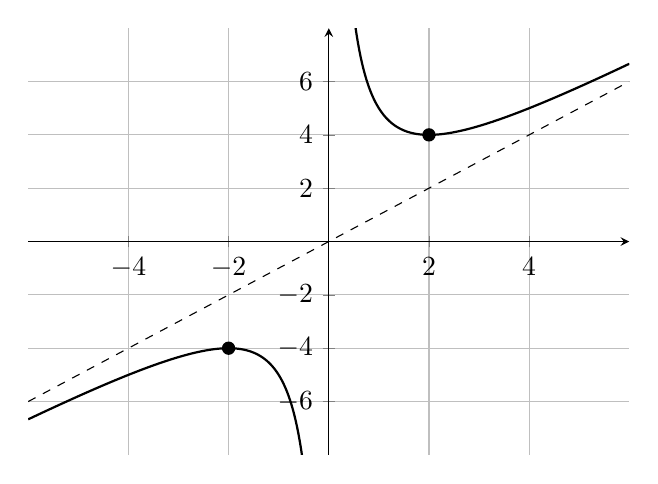
\begin{tikzpicture}
\begin{axis}[
  width=0.76\textwidth,
  height=7cm,
  axis lines=middle,
  xmin=-6,
  xmax=6,
  ymin=-8,
  ymax=8,
  grid=both,
  samples=200,
  xtick={-4,-2,2,4},
  ytick={-6,-4,-2,2,4,6}
]
\addplot[black, thick, domain=-6:-0.35] {x + 4/x};
\addplot[black, thick, domain=0.35:6] {x + 4/x};
\addplot[black, dashed, domain=-6:6] {x};
\addplot[black, dashed] coordinates {(0,-8) (0,8)};
\addplot[only marks, mark=*, mark size=2.2pt] coordinates {(-2,-4) (2,4)};
\end{axis}
\end{tikzpicture}
\end{center}

\begin{shortanswer}{[CH-R10-01]}
Dominio \(\R\setminus\{0\}\), asintotas \(x=0\) e \(y=x\), crecimiento en
\((-\infty,-2)\cup(2,\infty)\), decrecimiento en \((-2,0)\cup(0,2)\), maximo local
\((-2,-4)\), minimo local \((2,4)\), tangente en \(x=2\): \(y=4\).
\end{shortanswer}

\begin{fullsolution}{[CH-R10-01]}
El dominio es
\[
D_f=\R\setminus\{0\}.
\]

La funcion presenta asintota vertical en \(x=0\) porque el termino \(\dfrac{4}{x}\) diverge al
aproximarse al origen. Ademas,
\[
f(x)-x=\frac{4}{x}\longrightarrow 0 \quad \text{cuando } x\to \pm \infty,
\]
asi que la asintota oblicua es
\[
y=x.
\]

Para la monotonia derivamos:
\[
f'(x)=1-\frac{4}{x^2}=\frac{x^2-4}{x^2}.
\]
Como \(x^2>0\) para \(x\neq 0\), el signo depende de \(x^2-4=(x-2)(x+2)\). Por tanto,
\[
f'(x)>0 \text{ en }(-\infty,-2)\cup(2,\infty),
\]
\[
f'(x)<0 \text{ en }(-2,0)\cup(0,2).
\]
Se obtiene un maximo local en \(x=-2\) y un minimo local en \(x=2\). Sus valores son
\[
f(-2)=-2+\frac{4}{-2}=-4,\qquad f(2)=2+\frac{4}{2}=4.
\]

La tangente en \(x=2\) tiene pendiente
\[
f'(2)=1-\frac{4}{4}=0,
\]
de modo que es horizontal y pasa por \((2,4)\). Su ecuacion es
\[
y=4.
\]
\end{fullsolution}

\begin{selfcheck}
\begin{itemize}
  \item Distingo entre fallar una cuenta y elegir mal el metodo.
  \item Puedo pasar de un bloque aislado a un simulacro mixto sin perder el hilo.
  \item Reconozco que el reto final combina dominio, asintotas, derivada y tangente.
\end{itemize}
\end{selfcheck}
